\section{Anergy nets Switzerland}
\label{as:anergy_suisse}
\begin{landscape}
\begin{table}[h]
\centering
\caption{District energy systems in Switzerland ~\cite{energieschweizFallbeispieleThermischeNetze2018}; \textit{n/a}: not available}\vspace{2mm} 
\label{tab:anergieCH1} 
\begin{tabular}{llllllll}
\toprule
                                                                               & \textbf{\begin{tabular}[c]{@{}l@{}}Anergienetz \\ ETH \\ Hönggerberg\end{tabular}} & \textbf{\begin{tabular}[c]{@{}l@{}}Jardins de \\ la Pâla\end{tabular}}      & \textbf{\begin{tabular}[c]{@{}l@{}}Suurstoffi-\\ Areal\end{tabular}}                                  & \textbf{\begin{tabular}[c]{@{}l@{}}Anergienetz \\ Friesenberg (FGZ)\end{tabular}} & \textbf{\begin{tabular}[c]{@{}l@{}}CAD La-\\ Tour-De-Peilz\end{tabular}} & \textbf{\begin{tabular}[c]{@{}l@{}}Anergienetz-\\ Visp\end{tabular}}  & \textbf{\begin{tabular}[c]{@{}l@{}}Genève-Lac-\\ Nations (GLN)\end{tabular}}  \\
                                                                               \midrule
\textbf{Location}                                                              & Zürich                                                                             & Bulle                                                                       & Rotkreuz                                                                                              & Zürich                                                                            & La-Tour-de-Peilz                                                         & Visp                                                                  & Genève                                                                        \\
\textbf{Year of construction}                                                  & 2012 - 2026                                                                        & 2012 - 2020                                                                 & 2010 - 2020                                                                                           & 2011-2050                                                                         & 2013 - 2015                                                              & 2007 - heute                                                          & 2008 - 2016                                                                   \\
\textbf{Type}                                                                  & $\leq$ 20 \si{\celsius}                                                                            & $\leq$ 20 \si{\celsius}                                                                     & $\leq$ 20 \si{\celsius}                                                                                               & $\leq$ 20 \si{\celsius}                                                                           & $\leq$ 20\si{\celsius}                                                                   & $\leq$ 20 \si{\celsius}                                                               & $\leq$ 20 \si{\celsius}                                                                       \\
\textbf{Energy Ref. Area $[m2]$}                                                              & 475'000                                                                            & 65‘000                                                                      & 172'421                                                                                               & 185'000                                                                           & 24 Buildings                                                             & 160'000                                                               & 840'000                                                                       \\
\textbf{Use}                                                                   & \begin{tabular}[c]{@{}l@{}}School\\ Residential\end{tabular}                       & \begin{tabular}[c]{@{}l@{}}Residential\\ Commercial\\ Industry\end{tabular} & \begin{tabular}[c]{@{}l@{}}Residential\\ Administration\\ Commercial\\ Catering\\ School\end{tabular} & \begin{tabular}[c]{@{}l@{}}Residential\\ Computation\end{tabular}                 & \begin{tabular}[c]{@{}l@{}}Residential\\ Administration\end{tabular}     & \begin{tabular}[c]{@{}l@{}}Residential\\ Industry\end{tabular}        & \begin{tabular}[c]{@{}l@{}}Residential\\ Administration\\ School\end{tabular} \\
\textbf{Status}                                                                & Partly built                                                                       & Partly built                                                                & Partly built                                                                                          & Partly built                                                                      & Built                                                                    & Built                                                                 & Built                                                                         \\
\midrule
\textbf{}                                                                      & \multicolumn{7}{c}{Data Energy Consumption}                                                                                                                                                                                                                                                                                                                                                                                                                                                                                                                                                     \\
\midrule
\textbf{\begin{tabular}[c]{@{}l@{}}Inst. Heating\\ capacity $[kW]$\end{tabular}} & 8'000                                                                              & 2'000                                                                       & 6'732                                                                                                 & 3'930                                                                             & 10'000                                                                   & 3'467                                                                 & 4'300                                                                         \\
\textbf{\begin{tabular}[c]{@{}l@{}}Heating demand \\ $[MWh/a]$\end{tabular}}   & 28'450                                                                             & 3'100                                                                       & 10'619                                                                                                & 35'000                                                                            & 812                                                                      & 8'737                                                                 & 5’000                                                                         \\
\textbf{\begin{tabular}[c]{@{}l@{}}Inst. Cooling\\ capacity $[kW]$\end{tabular}} & 6'000                                                                              & 1'000                                                                       & 2'327                                                                                                 & 3'500                                                                             & None                                                                     & 2'600                                                                 & 16'200                                                                        \\
\textbf{\begin{tabular}[c]{@{}l@{}}Cooling demand \\ $[MWh/a]$\end{tabular}}   & 26'200                                                                             & 650                                                                         & 2'364                                                                                                 & 80'000                                                                            & None                                                                     & 3'380                                                                 & 20'000                                                                        \\
\textbf{Heat source}                                                           & \begin{tabular}[c]{@{}l@{}}Laboratories\\ waste heat \\ +HP\end{tabular}           & Groundwater+HP                                                              & \begin{tabular}[c]{@{}l@{}}Waste heat \\ buildings \\ + PVT (solar th.) \\ +HP\end{tabular}           & \begin{tabular}[c]{@{}l@{}}Waste heat\\ data center+HP\end{tabular}               & Lake water +HP                                                           & \begin{tabular}[c]{@{}l@{}}Inudstrial waste \\ heat + HP\end{tabular} & Lake water +HP                                                                \\
\textbf{Heat storage}                                                          & \begin{tabular}[c]{@{}l@{}}Geothermal well \\ field\\ (431 at 200m)\end{tabular}   & Groundwater 12\si{\celsius}                                                            & \begin{tabular}[c]{@{}l@{}}Geothermal well\\ field \\ (215 at 150 m,\\ 180 at 280m)\end{tabular}      & \begin{tabular}[c]{@{}l@{}}Geothermal well\\ field\\ (332 at 250m)\end{tabular}   & None                                                                     & None                                                                  & None                                                                          \\
\midrule
\textbf{}                                                                      & \multicolumn{7}{c}{Network data}                                                                                                                                                                                                                                                                                                                                                                                                                                                                                                                                                                \\
\midrule
\textbf{Network length $[km]$}                                                   & 1.5                                                                                & 0.85                                                                        & 2.5                                                                                                   & 1.5                                                                               & 4.1                                                                      & 4.2                                                                   & 6                                                                             \\
\textbf{Heating pipeT}                                                         & 24 \si{\celsius} - 8 \si{\celsius}                                                                       & 12 \si{\celsius} - 9 \si{\celsius}                                                                & 25 \si{\celsius} - 8 \si{\celsius}                                                                                          & 28 \si{\celsius} - 8 \si{\celsius}                                                                      & 20 \si{\celsius} - 6 \si{\celsius}                                                             & 18 \si{\celsius} - 8 \si{\celsius}                                                          & 17 \si{\celsius} - 5 \si{\celsius}                                                                  \\
\textbf{Cooling pipeT}                                                         & 4 \si{\celsius} - 20 \si{\celsius}                                                                       & 4 \si{\celsius} - 17 \si{\celsius}                                                                & 4 \si{\celsius} - 17 \si{\celsius}                                                                                          & 4 \si{\celsius} -24 \si{\celsius}                                                                       & 2 \si{\celsius} - 16 \si{\celsius}                                                             & 4 \si{\celsius} - 16 \si{\celsius}                                                          & 5 \si{\celsius} - 12 \si{\celsius}                                                                  \\
\textbf{Pipe diameter $[mm]$}                                                    & DN 560                                                                             & 75 - 250                                                                    & 60 - 400                                                                                              & 400 - 500                                                                         & 400 -700                                                                 & DN 400                                                                & 100 -700                                                                      \\
\textbf{Number of pipes}                                                       & 3                                                                                  & 2                                                                           & 2                                                                                                     & 2                                                                                 & 2                                                                        & 2                                                                     & 2       \\
\bottomrule
\end{tabular}
\end{table}

\end{landscape}
\begin{landscape}
\begin{table}[h]
\centering
\caption{District energy systems in Switzerland}\vspace{2mm}
\label{tab:anergieCH2} 
\begin{tabular}{llllllll}
\toprule

                                                                                      & \textbf{\begin{tabular}[c]{@{}l@{}}Anergienetz \\ ETH \\ Hönggerberg\end{tabular}} & \textbf{\begin{tabular}[c]{@{}l@{}}Jardins de \\ la Pâla\end{tabular}}             & \textbf{\begin{tabular}[c]{@{}l@{}}Suurstoffi-\\ Areal\end{tabular}} & \textbf{\begin{tabular}[c]{@{}l@{}}Anergienetz \\ Friesenberg (FGZ)\end{tabular}} & \textbf{\begin{tabular}[c]{@{}l@{}}CAD La-\\ Tour-De-Peilz\end{tabular}}      & \textbf{\begin{tabular}[c]{@{}l@{}}Anergienetz-\\ Visp\end{tabular}} & \textbf{\begin{tabular}[c]{@{}l@{}}Genève-Lac-\\ Nations (GLN)\end{tabular}} \\
                                                                                      \midrule
\textbf{}                                                                             & \multicolumn{7}{c}{Financial data}                                                                                                                                                                                                                                                                                                                                                                                                                                                                                                                                       \\
\midrule
\textbf{\begin{tabular}[c]{@{}l@{}}Tot. investments\\ '[Mio.CHF]'\end{tabular}}       & 37                                                                                 & 6                                                                                  & n/a                                                                  & 42.5                                                                              & 32                                                                            & 1.26                                                                 & 33                                                                           \\
\textbf{Interest rate[\%]}                                                            & 3.9 - 6.7                                                                          &                                                                                    & n/a                                                                  & n/a                                                                               & 6.4                                                                           & 5.8 - 8                                                              & n/a                                                                          \\
\textbf{Lifespan [a]}                                                                 &                                                                                    &                                                                                    &                                                                      &                                                                                   &                                                                               &                                                                      &                                                                              \\
\textbf{Pipes}                                                                        & 50                                                                                 & 30                                                                                 & 40                                                                   & 50                                                                                & 50                                                                            & 40                                                                   & n/a                                                                          \\
\textbf{Storage}                                                                      & 50                                                                                 & None                                                                               & 80                                                                   & 50                                                                                & None                                                                          & None                                                                 & n/a                                                                          \\
\textbf{Heating unit}                                                                 & 20                                                                                 & 15                                                                                 & 20                                                                   & 20                                                                                & 25                                                                            & 20                                                                   & n/a                                                                          \\
\textbf{Cooling unit}                                                                 & 20                                                                                 & 15                                                                                 & 20                                                                   & 20                                                                                & 25                                                                            & 20                                                                   & n/a                                                                          \\
\textbf{\begin{tabular}[c]{@{}l@{}}Cost of energy \\ '[Rp./kWh]'\end{tabular}}        & \begin{tabular}[c]{@{}l@{}}7.7 \\ (Heating +cooling)\end{tabular}                  & \begin{tabular}[c]{@{}l@{}}5.85 – 8\\ (at the moment \\ only heating)\end{tabular} & n/a                                                                  & \begin{tabular}[c]{@{}l@{}}18\\ (Heating)\end{tabular}                            & \begin{tabular}[c]{@{}l@{}}19.8\\ (at the moment\\ only heating)\end{tabular} & \begin{tabular}[c]{@{}l@{}}22.9\\ (Heating +\\ cooling)\end{tabular} & n/a                                                                          \\
\textbf{Tot. COP of heating}                                                          & 7.2                                                                                & 4.4                                                                                & n/a                                                                  & 5.2                                                                               & n/a                                                                           & n/a                                                                  & n/a                                                                          \\
\textbf{\begin{tabular}[c]{@{}l@{}}Tot. COP of heating\\ (incl. Pumps…)\end{tabular}} & 5.8                                                                                & 2.7                                                                                & 2.7                                                                  & 4.1                                                                               & 3.5-4                                                                         & 4                                                                    & 6.5                                                                          \\
\textbf{Tot. EER of cooling}                                                          & 30.1                                                                               & n/a                                                                                & n/a                                                                  & n/a                                                                               & n/a                                                                           & n/a                                                                  & n/a                                                                          \\
\textbf{\begin{tabular}[c]{@{}l@{}}Tot. EER of cooling\\ (incl. Pumps…)\end{tabular}} & 6.9                                                                                & 12.1                                                                               & n/a                                                                  & n/a                                                                               & n/a                                                                           & n/a                                                                  & n/a \\
\bottomrule
\end{tabular}
\end{table}

\end{landscape}
\clearpage
\newpage
\section{Call for tender Eglantine - details}
\label{as:eglantine}
\begin{table}[h!]
\centering
\caption{Estimated energy demand in call for tender}\vspace{2mm}
\label{tab:ppa_summary} 
\begin{tabular}{lrrrrr}
\toprule
\textbf{Building} & \begin{tabular}[c]{@{}l@{}}\textbf{Energy Ref.} \\ \textbf{Area (ERA)}\end{tabular} & \textbf{Inhabitants} & \begin{tabular}[c]{@{}l@{}}\textbf{Space Heating} \\ \textbf{(SH)}\end{tabular}                                             & \begin{tabular}[c]{@{}l@{}}\textbf{Hot Water} \\ \textbf{(DHW)}\end{tabular} & \textbf{TOTAL}     \\
         &                                                                        &             & \begin{tabular}[c]{@{}l@{}}MIINERGIE\\ simple flux\end{tabular} & SIA 380/1       &           \\
         & [m2]                                                                   &             & [kWh/yr]                                                        & [kWh/yr]        & [kWh/yr]  \\
         \midrule
1        & 8'200                                                                  & 273         & 245'180                                                         & 170'833         & 416'013   \\
2        & 2'615                                                                  & 76          & 82'308                                                          & 50'104          & 132'412   \\
3        & 2'415                                                                  & 70          & 76'328                                                          & 45'938          & 122'266   \\
4        & 2'780                                                                  & 92          & 83'122                                                          & 57'917          & 141'039   \\
5        & 3'700                                                                  & 116         & 113'246                                                         & 74'306          & 187'552   \\
6        & 1'500                                                                  & 50          & 44'850                                                          & 31'250          & 76'100    \\
7        & 2'870                                                                  & 83          & 90'652                                                          & 54'653          & 145'305   \\
8        & 2'500                                                                  & 83          & 74'750                                                          & 52'083          & 126'833   \\
9        & 4'225                                                                  & 140         & 126'328                                                         & 88'021          & 214'349   \\
10       & 4'455                                                                  & 148         & 133'205                                                         & 92'813          & 226'018   \\
11       & 4'190                                                                  & 139         & 125'281                                                         & 87'292          & 212'573   \\
12       & 2'300                                                                  & 76          & 68'770                                                          & 47'917          & 116'687   \\
13       & 2'300                                                                  & 76          & 68'770                                                          & 47'917          & 116'687   \\
14       & 2'300                                                                  & 76          & 68'770                                                          & 47'917          & 116'687   \\
\midrule
\textbf{TOT}      & \textbf{46'350}                              & \textbf{1'498}       & \textbf{1'401'559}      & \textbf{948'958}         & \textbf{2'350'521} \\
\bottomrule
\end{tabular}
\end{table}
\begin{table}[h!]
\centering
\caption{Estimated use of buildings in call for tender}\vspace{2mm}
\label{tab:ppa_buildinguse}
\begin{tabular}{lllll}
\toprule
\textbf{Building} & \textbf{Multidwelling} & \textbf{Retail} & \textbf{Restaurant services} & \textbf{Indoor swimming pool} \\
                  & \textbf{[\%]}               & \textbf{[\%]}      & \textbf{[\%]}          & \textbf{[\%]}              \\
                  \midrule
\textbf{1}        & 89.58\%                     & 3.10\%             & 4.42\%                 & 2.89\%                     \\
\textbf{2}        & 97.54\%                     & 2.46\%             & 0.00\%                 & 0.00\%                     \\
\textbf{3}        & 100.00\%                    & 0.00\%             & 0.00\%                 & 0.00\%                     \\
\textbf{4}        & 100.00\%                    & 0.00\%             & 0.00\%                 & 0.00\%                     \\
\textbf{5}        & 93.19\%                     & 6.81\%             & 0.00\%                 & 0.00\%                     \\
\textbf{6}        & 95.79\%                     & 4.21\%             & 0.00\%                 & 0.00\%                     \\
\textbf{7}        & 95.79\%                     & 4.21\%             & 0.00\%                 & 0.00\%                     \\
\textbf{8}        & 100.00\%                    & 0.00\%             & 0.00\%                 & 0.00\%                     \\
\textbf{9}        & 100.00\%                    & 0.00\%             & 0.00\%                 & 0.00\%                     \\
\textbf{10}       & 100.00\%                    & 0.00\%             & 0.00\%                 & 0.00\%                     \\
\textbf{11}       & 100.00\%                    & 0.00\%             & 0.00\%                 & 0.00\%                     \\
\textbf{12}       & 100.00\%                    & 0.00\%             & 0.00\%                 & 0.00\%                     \\
\textbf{13}       & 100.00\%                    & 0.00\%             & 0.00\%                 & 0.00\%                     \\
\textbf{14}       & 100.00\%                    & 0.00\%             & 0.00\%                 & 0.00\%                     \\ \midrule
\textbf{Tot}	  & 97.08 \%					& 1.63 \%			& 0.78 \%					& 0.51 \%					\\
\bottomrule
\end{tabular}
\end{table}
\begin{table}[h!]
\centering
\caption{Estimated sizing of energy system in call for tender}\vspace{2mm}
\label{tab:ppa_prestudy} 
\begin{tabular}{lllll}
\toprule
\textbf{Building} & \textbf{PV}    & \textbf{HP}    & \multicolumn{2}{l}{\textbf{Geothermal}} \\
         &       &       & \textbf{Nb. wells}        & \textbf{Depth}        \\
         & \textbf{[kWp]} & \textbf{[kW] } &                 & \textbf{[m] }         \\
         \midrule
1        & 46    & 223   & 13              & 284          \\
2        & 45    & 70    & 4               & 291          \\
3        & 35    & 64    & 4               & 269          \\
4        & 33    & 76    & 5               & 250          \\
5        & 49    & 100   & 6               & 276          \\
6        & 55    & 41    & 3               & 225          \\
7        & 55    & 77    & 5               & 256          \\
8        & 37    & 68    & 4               & 281          \\
9        & 66    & 115   & 7               & 271          \\
10       & 0     & 121   & 7               & 286          \\
11       & 59    & 114   & 7               & 269          \\
12       & 33    & 63    & 4               & 259          \\
13       & 32    & 63    & 4               & 259          \\
14       & 27    & 63    & 4               & 267          \\
\midrule
\textbf{TOT}      & \textbf{570}   & \textbf{1'258} & \textbf{77}              &             \\
\bottomrule
\end{tabular}
\end{table}
\begin{figure}[htp]
	\centering
	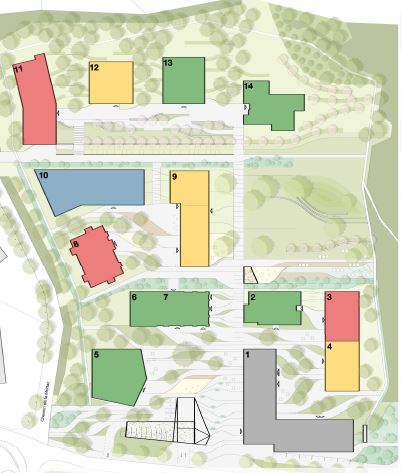
\includegraphics[width=0.45\textwidth]{ppa_buildings.JPG}
	\caption{Map of the planned Eglantine district}
	\label{fig:ppa_buildings}
\end{figure}
\clearpage
\newpage
\section{CO2DEN}\label{as:co2den}
\begin{figure}[htp]
	\centering
	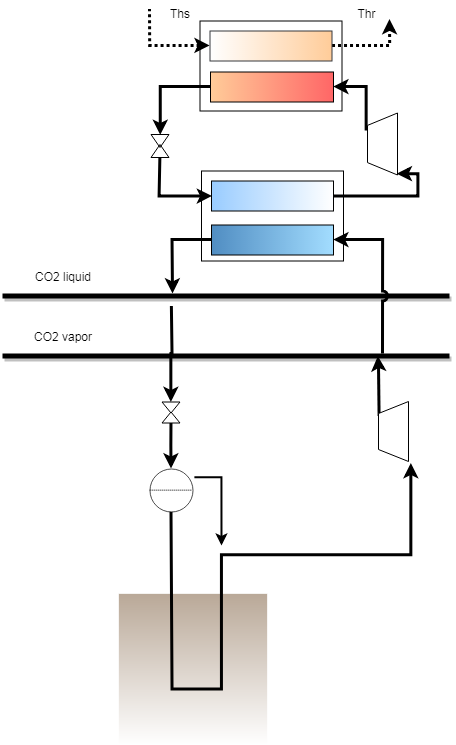
\includegraphics[width=0.3\textwidth]{CO2-DX-GSHP.png}
	\caption{A simplified schematics of the CO2 DEN with DX-GSHP technology}
	\label{fig:co2_gshp}
\end{figure}
\clearpage
\newpage
\section{Geothermal analysis for the Lemanic region} \label{as:gt}
\begin{figure}[tph]
	\centering
	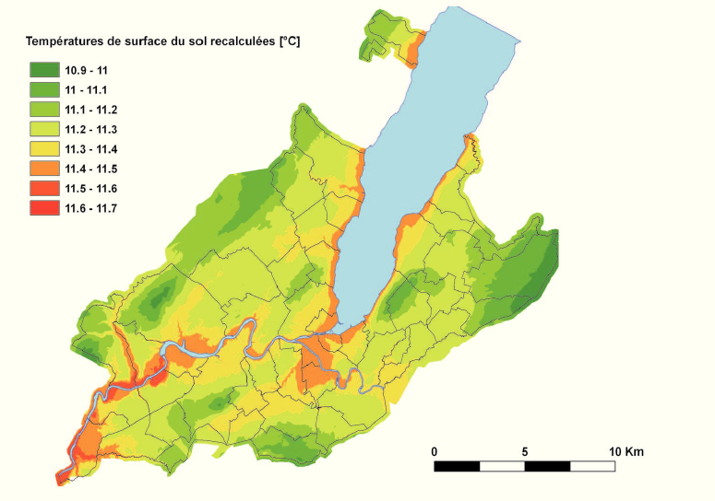
\includegraphics[width=0.8\linewidth]{GTW_Ts}
	\caption{Surface temperature in the Lemanic region. Source:~\cite{gadzEvaluationPotentielGeothermique2011}}
	\label{fig:gtwts}
\end{figure}
\begin{figure}[tph]
	\centering
	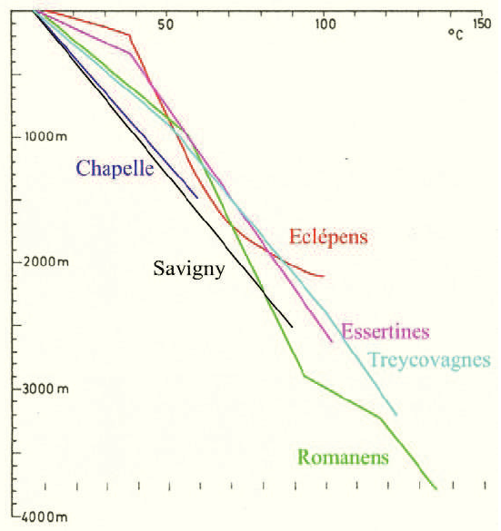
\includegraphics[width=0.6\linewidth]{GTW_grad}
	\caption{Temperature gradient in the ground, in function of depth, in the Lemanic region. Source: ~\cite{gadzEvaluationPotentielGeothermique2011}}
	\label{fig:gtwgrad}
\end{figure}

\clearpage
\newpage
\section{Geothermal models}\label{as:gtw}
\begin{figure}[tph]
	\centering
	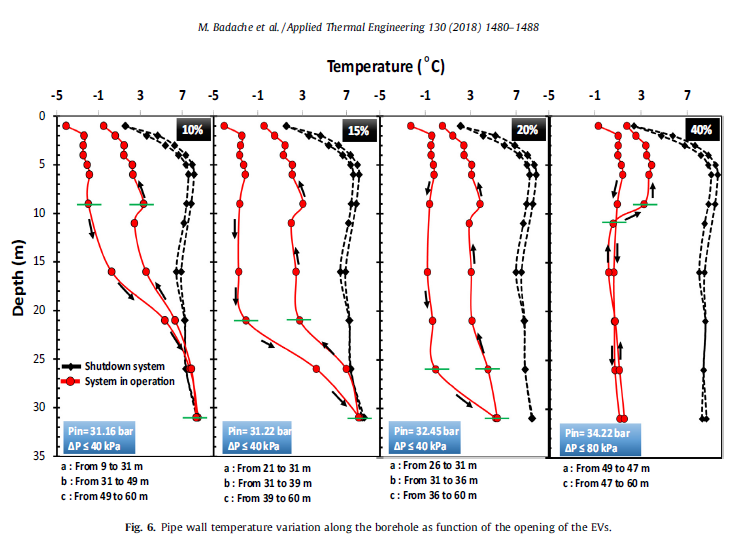
\includegraphics[width=0.7\linewidth]{Images/gtw_model1}
	\caption{Pipe wall temperature variation along the borehole as function of the opening of the expansion valve, in a direct expansion GSHP. Source: ~\cite{badacheExperimentalStudyCarbon2018}}
	\label{fig:gtwmodel1}
\end{figure}
\begin{figure}[tph]
	\centering
	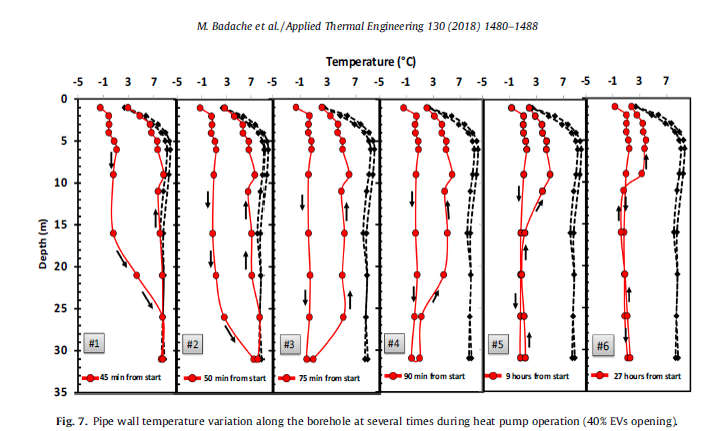
\includegraphics[width=0.7\linewidth]{Images/gtw_model2}
	\caption{Pipe walll temperature variation along the borehole at several times during heat pump operation, in a direct expansion GSHP. Source: ~\cite{badacheExperimentalStudyCarbon2018}}
	\label{fig:gtwmodel2}
\end{figure}

